\chapter{Contas Públicas}
\section{Receitas do Governo}
	
\lipsum[1-2]
	
\begin{figure}[h]
	\caption{Titulo}
	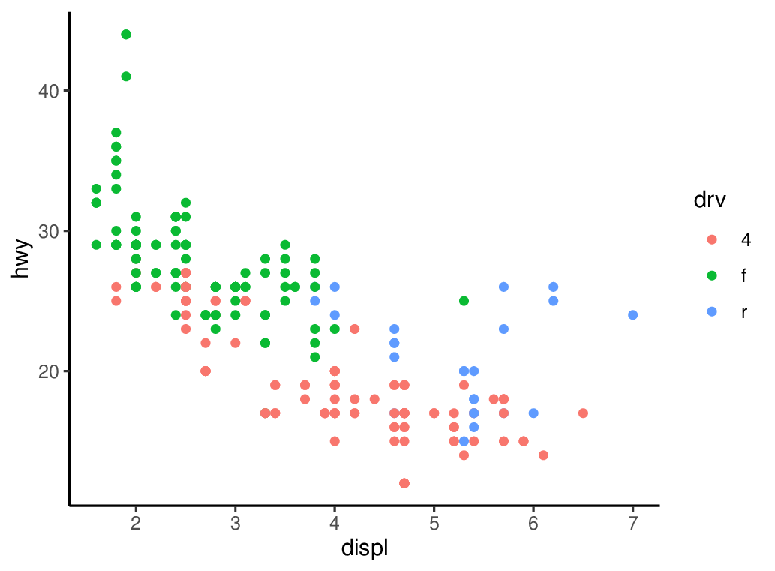
\includegraphics[width=\linewidth]{fig/plot}
	\source{mpg, EUA}
	\notes{Aqui inseri mais notas explicativas}
\end{figure}
	
\lipsum[1]
	
\begin{bbox}{Informações Longa}
	\lipsum[1-2]
\end{bbox}
	
\section{Despesas do Governo}
	
\lipsum[1-2]
	
\begin{figure}[h]
	\caption{Exemplo Com Duas Figura}
	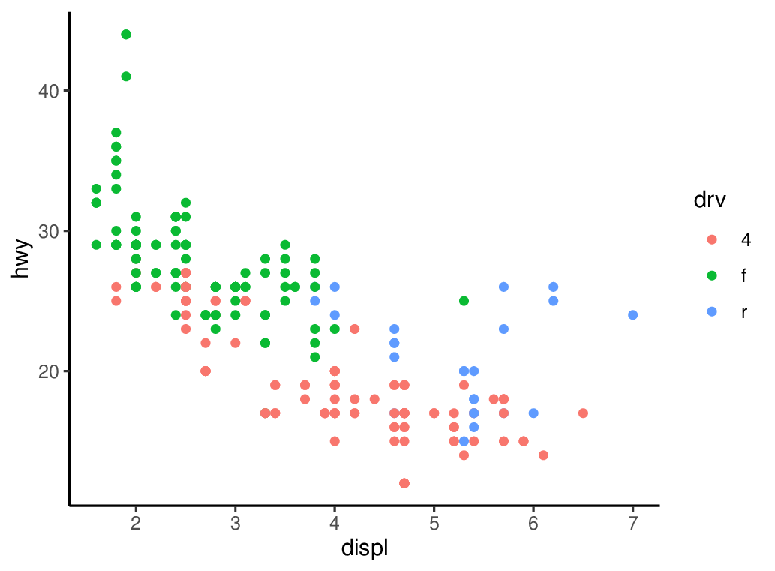
\includegraphics[width=\linewidth]{fig/plot}
	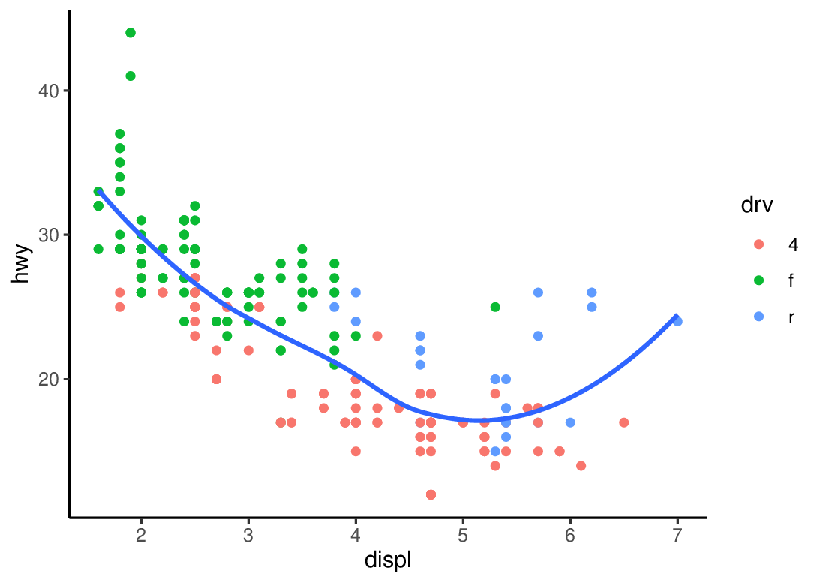
\includegraphics[width=\linewidth]{fig/plot2}
	\source{mpg, EUA}
	\notes{Aqui inseri mais notas explicativas}
\end{figure}

\section{Despesas por Poder}

\lipsum[1-2]

\begin{smbox}{Informações Curtas}
	\lipsum[1]
\end{smbox}

\lipsum[1]

\begin{figure}[h]
	\caption{Exemplo Com Duas Subfiguras}
	\begin{subfigure}[t]{0.5\textwidth}
		\caption{Título Subfigura}
		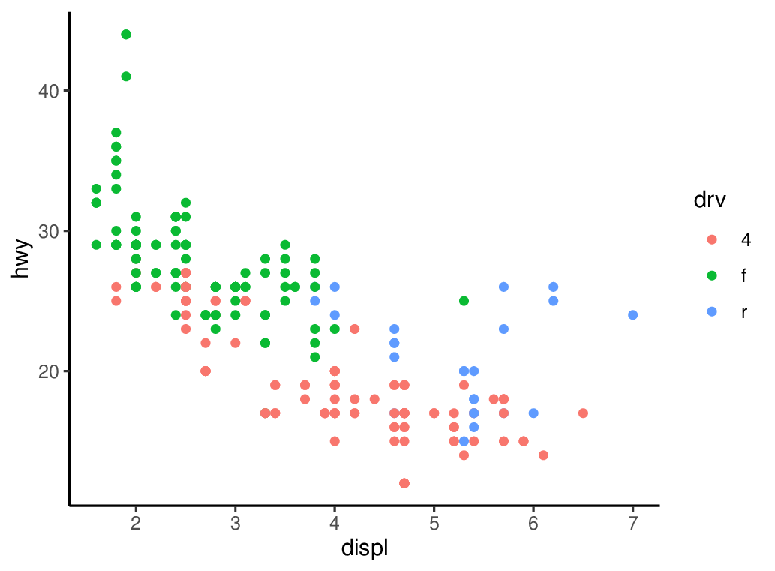
\includegraphics[width=\linewidth]{fig/plot}
	\end{subfigure}
	\begin{subfigure}[t]{0.5\textwidth}
		\caption{Título Subfigura}
		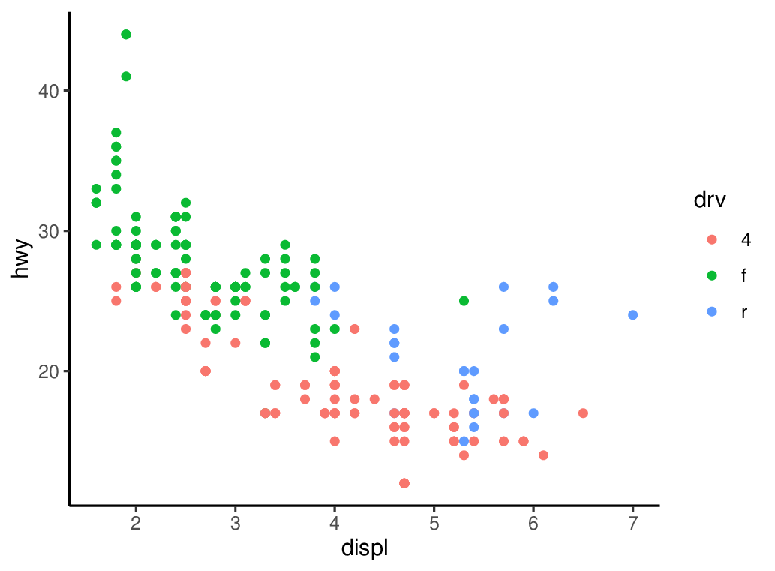
\includegraphics[width=\linewidth]{fig/plot}
	\end{subfigure}
	\source{mpg, EUA}
	\notes{Aqui inseri mais notas explicativas}
\end{figure}

\lipsum[1-5]

\begin{figure*}[h]
	\caption{Quadro de Figuras}
	\begin{subfigure}[h]{0.5\textwidth}
		\caption{Título Subfigura}
		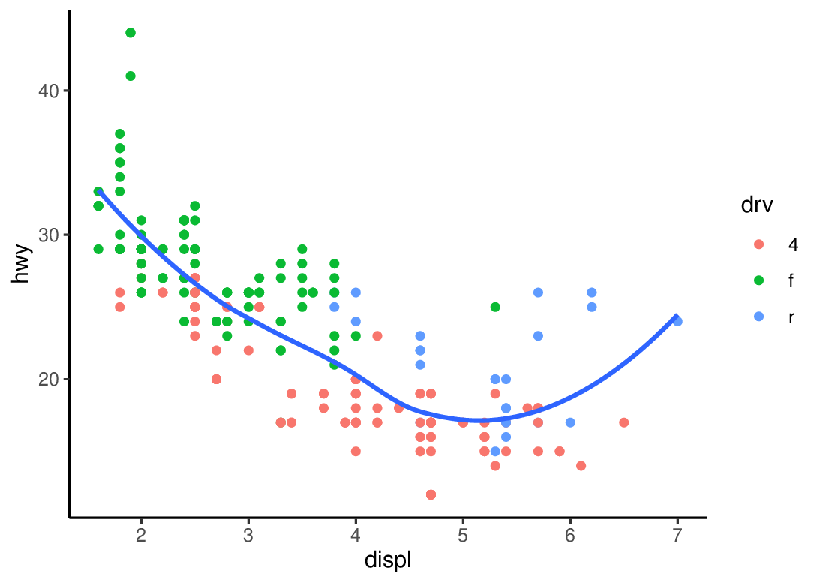
\includegraphics[width=\linewidth]{fig/plot2}
	\end{subfigure}
	\begin{subfigure}[h]{0.5\textwidth}
		\caption{Título Subfigura}
		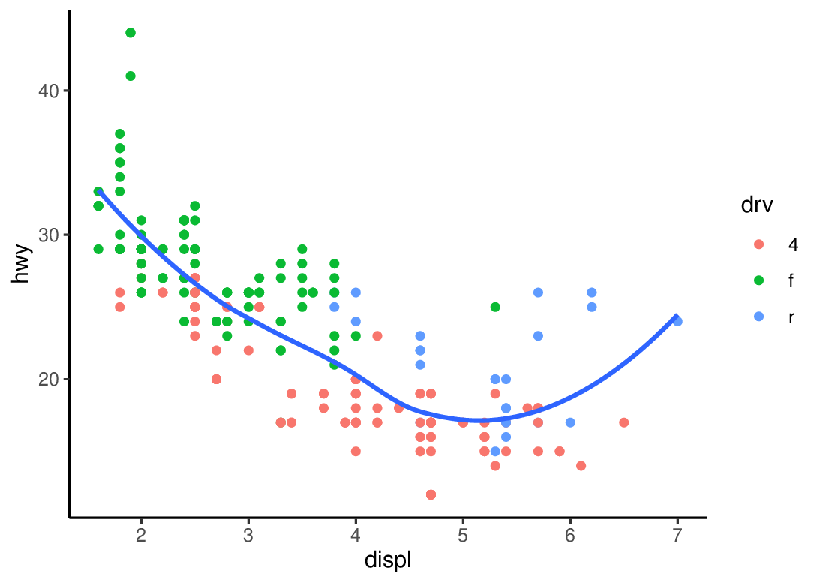
\includegraphics[width=\linewidth]{fig/plot2}
	\end{subfigure}
	\begin{subfigure}[h]{0.5\textwidth}
		\caption{Título Subfigura}
		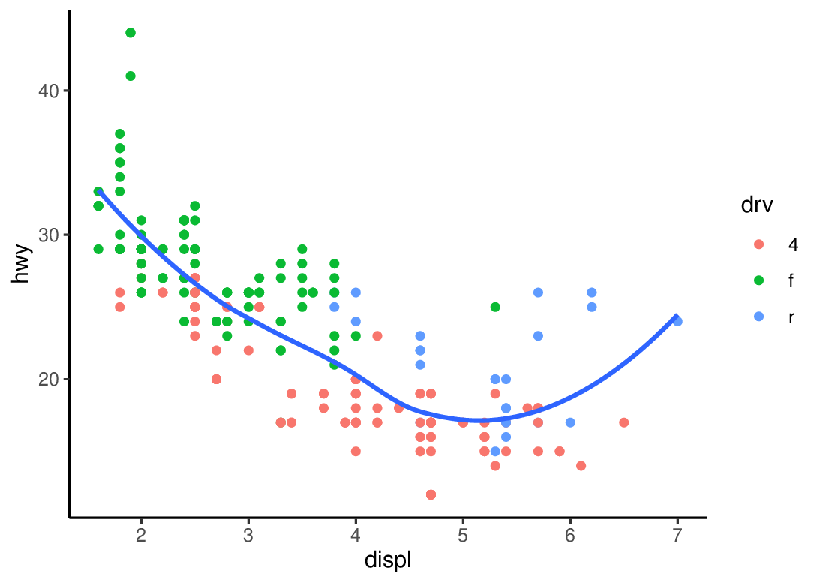
\includegraphics[width=\linewidth]{fig/plot2}
	\end{subfigure}
	\begin{subfigure}[h]{0.5\textwidth}
		\caption{Título Subfigura}
		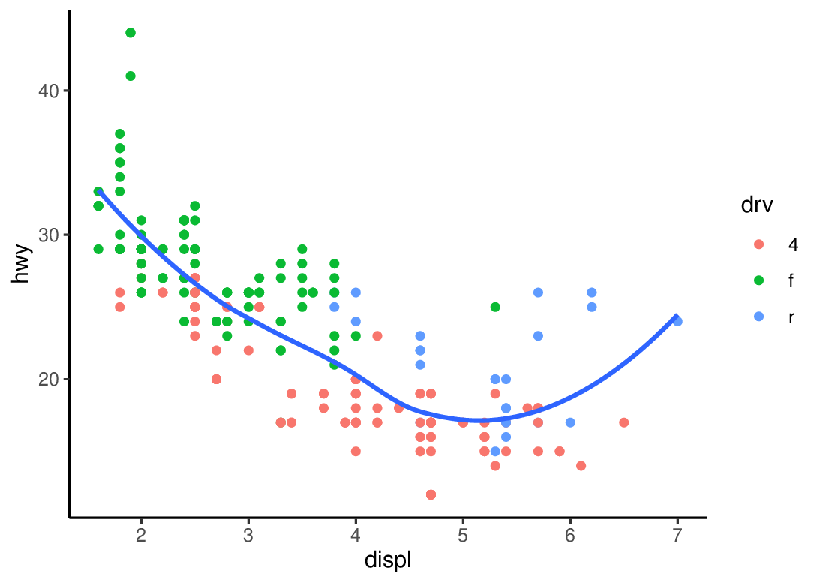
\includegraphics[width=\linewidth]{fig/plot2}
	\end{subfigure}
	\source{mpg, EUA}
	\notes{Aqui inseri mais notas explicativas}
\end{figure*}
